\documentclass[12pt]{article}
\usepackage{preamble}
\graphicspath{{pics/ps1a/}}
\begin{document}
% \maketitle
\lhead{Problem Set 1a}

%%%%%%%%%%%%%%%%%%%%%%%%%%%%%%%%%%%%%%%%%%%%%%%
%                  Definitions                %
%%%%%%%%%%%%%%%%%%%%%%%%%%%%%%%%%%%%%%%%%%%%%%%
%\includegraphics[width=\mywidth\textwidth]{}

% \begin{figure}[h!]
% \centering
% \input{pics/PS2/p7b}
% \caption{}
% \label{fig-}
% \end{figure}

% \begin{enumerate}[label=\alph*.]
%     \setcounter{enumi}{1}
%     \item 
% \end{enumerate}
\renewcommand{\vem}{\newpage}


%%%%%%%%%%%%%%%%%%%%%%%%%%%%%%%%%%%%%%%%%%%%%%%
%                Problem 1                    %
%%%%%%%%%%%%%%%%%%%%%%%%%%%%%%%%%%%%%%%%%%%%%%%
\problem{1.*Let it Snow!}{
Before getting started with the data work, first consider the table from Snow (1855)
reproduced in the lecture notes (“Snow’s Table IX”). The table reports only means.
\begin{enumerate}[label=(\alph*)]
    \item Develop an approximate 95\% confidence interval for ``Deaths per 10,000 Houses'' for Southwark and Vaxhall customers. Develop another 95\% CI for the same quantity for Lambeth. Do the confidence intervals overlap?
    \end{enumerate} 
}

\begin{figure}[h!]
\centering
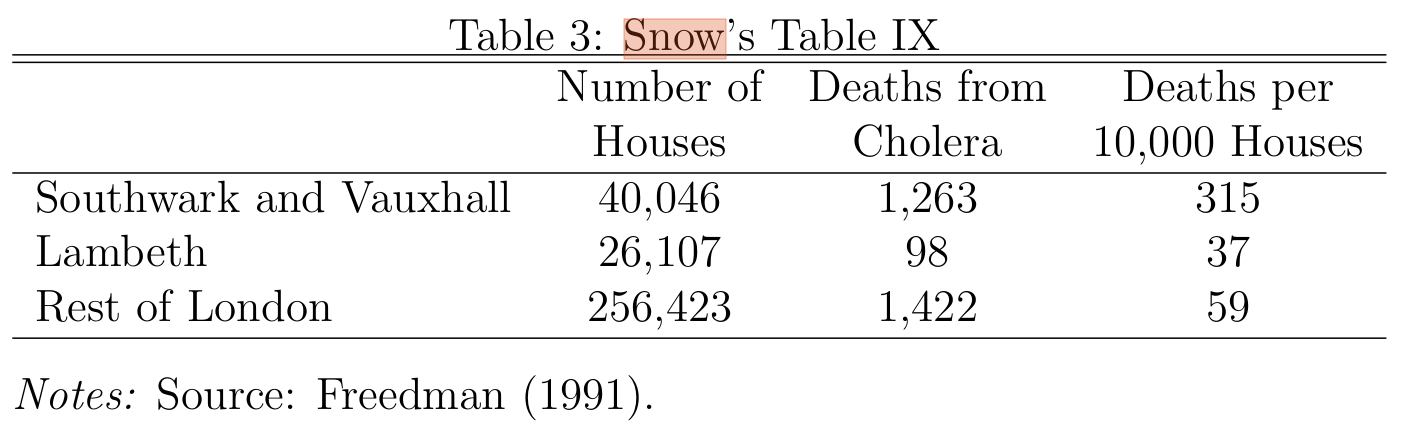
\includegraphics[width=0.8\textwidth]{snow_table}
\label{fig-1}
\end{figure}

\begin{align*}
\intertext{Assuming that, within a region $k\in\{a, b, c\}$, the indicator of one person in household $i$ dying from Cholera $X^k_i$ is distributed as a Bernoulli random variable with probability $p_k$ -- $X^k_i\iid \text{Bernoulli}(p_k)$. Then deaths per 10,000 households in region $k$, $R_k$, is a function of the sum of i.i.d. Bernoulli random variables. Let $N_k$ be the number of houses in region $k$, then}
R_k &= \frac{10,000}{N_k}\sum\limits_{i=1}^{N_k}X^k_i 
    \sim  \frac{10,000}{N_k}\text{Binom}(N_k, p_k)
\intertext{Let $Z^k\sim\text{Binom}(N_k, p_k)$. Then the variance of $R_k$ is}
\text{var}(R_k) &= \text{var}(\frac{10,000}{N_k}Z^k) \\
    &= \left(\frac{10,000}{N_k}\right)^2\text{var}(Z^k) \\
    &= \left(\frac{10,000}{N_k}\right)^2 N_k\cdot p_k\cdot (1-p_k) \\
    &= \frac{(10,000)^2}{N_k} p_k(1-p_k) \\
\intertext{Let $ z_{\alpha}$ be the z-score at significance level $\alpha$. Then, for large enough $N_k$ (which 26,000 is probably large enough), the 95\% confidence interval for $R_k$ would be:}
\text{CI}_{95} &= R_k \pm z_{5\%}\sqrt{\text{var}(R_k)} \\
    &= R_k \pm z_{5\%}\sqrt{\frac{(10,000)^2}{N_k} p_k(1-p_k) } \\
    &= R_k \pm 10,000z_{5\%}\sqrt{\frac{p_k(1-p_k)}{N_k}} \\
\intertext{And an unbiased estimator for the probability of death $p_k$ would be the mean of the indicators:}
\hat{p}_k &= \frac{1}{N_k}\sum\limits_{i=1}^{N_k}X^k_i = \overline{X^k_i}
\end{align*}

Calculating $\hat{p}_k$ from the Snow table, we get
\begin{table}[h!]
\centering
\begin{tabular}{|c|c|c|}
\hline
$R_k$ & CI$_k$ lower & CI$_k$ upper \\
\hline
      &              &              \\
\hline
      &              &             \\
\hline
\end{tabular}
\end{table}


%%%%%%%%%%%%%%%%%
%     Part b    %
%%%%%%%%%%%%%%%%%
\vem
\problem{}{
    \begin{enumerate}[label=(\alph*)]
    \setcounter{enumi}{1}
    \item Discuss either formally or intuitively the critical assumption that underlies your confidence intervals. Give a 2 or 3 sentence quote from Snow’s description (re-produced in Freedman (1991)) that supports this assumption.
    \end{enumerate} 
}





%%%%%%%%%%%%%%%%%
%     Part c    %
%%%%%%%%%%%%%%%%%
\vem
\problem{}{
We now move to some analysis of real data. The data portions of Problem Sets 1a and
1b are based heavily on the paper Almond, Chay, and Lee (2005), and problem sets from
Ken Chay and John DiNardo based on some of the data used in the paper. The goal of
this assignment is to examine the research question: what is the causal effect of maternal
smoking during pregnancy on infant birthweight and other infant health outcomes. The
data for the problem set is an extract of all births from the 1993 National Natality Detail
Files for Pennsylvania. Each observation represents an infant-mother match. The data in
Stata format can be downloaded from the bCourses website. There should be 48 variables
in the data and, after you are finished with the cleaning steps described below, 114,610
observations.\\

The data here are “real” and quite imperfect, which will help simulate the unpleasantness
of real world data work. Unlike the real world where you will confront this bleak situation
largely alone, I will provide you with some hints for working your way through the raw data.
You can download part of the codebook for the data to help you figure out the relevant
variables.
}



\newpage
%%%%%%%%%%%%%%%%%%%%%%%%%%%%%%%%%%%%%%%%%%%%%%%
%                Problem II                   %
%%%%%%%%%%%%%%%%%%%%%%%%%%%%%%%%%%%%%%%%%%%%%%%
\problem{2. Real Data}{
The first order of business is to go through the code book, decide on the relevant
variables, and process the data. This involves several steps:
\vem
    \begin{enumerate}[label=(\alph*)]
        \item Fix missing values. In the the data set several variables take on a value of, say, 9999 if missing. We have already checked for missing observations for about 2/3 of the variables. The remaining variables need to be checked and are the last 15 in the variable list (i.e. from ’cardiac’ to ’wgain’). Refer to the codebook for missing value codes. Produce an analysis data set that drops any observation with missing values.
    \end{enumerate} 
}






%%%%%%%%%%%%%%%%%
%     Part b   %
%%%%%%%%%%%%%%%%%
\vem
\problem{}{
    \begin{enumerate}[label=(\alph*)]
    \setcounter{enumi}{1}
        \item If this were a real research project you would want to consider other approaches to missing data besides termination with extreme prejudice. What observations do you have to drop because of missing data. Might this affect your results? Do the data appear to be missing completely at random? How might you assess whether the data appear to be missing at random?
    \end{enumerate} 
}




%%%%%%%%%%%%%%%%%
%     Part c   %
%%%%%%%%%%%%%%%%%
\vem
\problem{}{
    \begin{enumerate}[label=(\alph*)]
    \setcounter{enumi}{2}
        \item Produce a summary table describing the final analysis data set.
    \end{enumerate} 
}




\newpage
%%%%%%%%%%%%%%%%%%%%%%%%%%%%%%%%%%%%%%%%%%%%%%%
%                Problem 3                    %
%%%%%%%%%%%%%%%%%%%%%%%%%%%%%%%%%%%%%%%%%%%%%%%
\problem{3. Smoking and birth weight}{
The next part of the assignment is to try to estimate the “causal” effect of maternal
smoking during pregnancy on infant birth weight. Let’s start out using techniques that
are familiar, and think about whether they are likely to work in this context. Answer
the following questions.\\

    \begin{enumerate}[label=(\alph*)]
    \item Compute the mean difference in APGAR scores (both five and one minute versions) as well as birthweight by smoking status.
    \end{enumerate} 
}



%%%%%%%%%%%%%%%%%
%     Part b    %
%%%%%%%%%%%%%%%%%
\vem
\problem{}{
    \begin{enumerate}[label=(\alph*)]
    \setcounter{enumi}{1}
    \item Under what circumstances can one identify the average treatment effect of maternal smoking by comparing the unadjusted difference in mean birth weight of infants of smoking and non-smoking mothers? Estimate its impact under this assumption. Provide and comment on some evidence for or against the validity of the assumption (A useful “Table 1” of any paper is one that describes the overall averages of the observations, and then describes the subsets of people who do and do not receive the treatment (when it is binary)).
    \end{enumerate} 
}


%%%%%%%%%%%%%%%%%
%     Part c    %
%%%%%%%%%%%%%%%%%
\vem
\problem{}{
    \begin{enumerate}[label=(\alph*)]
    \setcounter{enumi}{2}
        \item Suppose that maternal smoking is randomly assigned conditional on the  other observable “predetermined” determinants of infant birth weight. First discuss which (if any) of the variables contained in the data set can clearly be considered to be predetermined. In general, what kinds of variables can be considered predetermined and what kinds of variables cannot?
    \end{enumerate} 
}


%%%%%%%%%%%%%%%%%
%     Part d    %
%%%%%%%%%%%%%%%%%
\vem
\problem{}{
    \begin{enumerate}[label=(\alph*)]
    \setcounter{enumi}{3}
        \item What does “selection on observables” impl y about the relationship between maternal smoking and unobservable determinants of birth weight conditional on the observables? Use a basic linear regression model, in conjunction with your answer to part (c), to estimate the impact of smoking and report your estimates. Under what circumstances is the average treatment effect identified?
    \end{enumerate} 
}


\end{document}

References
